\let\negmedspace\undefined
\let\negthickspace\undefined
%\RequirePackage{amsmath}
\documentclass[journal,12pt,twocolumn]{IEEEtran}
%
% \usepackage{setspace}
 \usepackage{gensymb}
%\doublespacing
 \usepackage{polynom}
%\singlespacing
%\usepackage{silence}
%Disable all warnings issued by latex starting with "You have..."
%\usepackage{graphicx}
\usepackage{amssymb}
%\usepackage{relsize}
\usepackage[cmex10]{amsmath}
%\usepackage{amsthm}
%\interdisplaylinepenalty=2500
%\savesymbol{iint}
%\usepackage{txfonts}
%\restoresymbol{TXF}{iint}
%\usepackage{wasysym}
\usepackage{amsthm}
%\usepackage{pifont}
%\usepackage{iithtlc}
% \usepackage{mathrsfs}
% \usepackage{txfonts}
 \usepackage{stfloats}
% \usepackage{steinmetz}
 \usepackage{bm}
% \usepackage{cite}
% \usepackage{cases}
% \usepackage{subfig}
%\usepackage{xtab}
\usepackage{longtable}
%\usepackage{multirow}
%\usepackage{algorithm}
%\usepackage{algpseudocode}
\usepackage{enumitem}
 \usepackage{mathtools}
 \usepackage{tikz}
% \usepackage{circuitikz}
% \usepackage{verbatim}
%\usepackage{tfrupee}
\usepackage[breaklinks=true]{hyperref}
%\usepackage{stmaryrd}
%\usepackage{tkz-euclide} % loads  TikZ and tkz-base
%\usetkzobj{all}
\usepackage{listings}
    \usepackage{color}                                            %%
    \usepackage{array}                                            %%
    \usepackage{longtable}                                        %%
    \usepackage{calc}                                             %%
    \usepackage{multirow}                                         %%
    \usepackage{hhline}                                           %%
    \usepackage{ifthen}                                           %%
  %optionally (for landscape tables embedded in another document): %%
    \usepackage{lscape}     
% \usepackage{multicol}
% \usepackage{chngcntr}
%\usepackage{enumerate}

%\usepackage{wasysym}
%\newcounter{MYtempeqncnt}
\DeclareMathOperator*{\Res}{Res}
\DeclareMathOperator*{\equals}{=}
%\renewcommand{\baselinestretch}{2}
\renewcommand\thesection{\arabic{section}}
\renewcommand\thesubsection{\thesection.\arabic{subsection}}
\renewcommand\thesubsubsection{\thesubsection.\arabic{subsubsection}}

\renewcommand\thesectiondis{\arabic{section}}
\renewcommand\thesubsectiondis{\thesectiondis.\arabic{subsection}}
\renewcommand\thesubsubsectiondis{\thesubsectiondis.\arabic{subsubsection}}

% correct bad hyphenation here
\hyphenation{op-tical net-works semi-conduc-tor}
\def\inputGnumericTable{}                                 %%

\lstset{
%language=C,
frame=single, 
breaklines=true,
columns=fullflexible
}
%\lstset{
%language=tex,
%frame=single, 
%breaklines=true
%}
\title{Assignment 2}
\author{K Vivek Kumar}

\begin{document}
\date{April 11,2022}
\maketitle
%
\newtheorem{theorem}{Theorem}[section]
\newtheorem{problem}{Problem}
\newtheorem{proposition}{Proposition}[section]
\newtheorem{lemma}{Lemma}[section]
\newtheorem{corollary}[theorem]{Corollary}
\newtheorem{example}{Example}[section]
\newtheorem{definition}[problem]{Definition}
%\newtheorem{thm}{Theorem}[section] 
%\newtheorem{defn}[thm]{Definition}
%\newtheorem{algorithm}{Algorithm}[section]
%\newtheorem{cor}{Corollary}
\newcommand{\BEQA}{\begin{eqnarray}}
\newcommand{\EEQA}{\end{eqnarray}}
\newcommand{\define}{\stackrel{\triangle}{=}}
\newcommand*\circled[1]{\tikz[baseline=(char.base)]{
    \node[shape=circle,draw,inner sep=2pt] (char) {#1};}}
\bibliographystyle{IEEEtran}
%\bibliographystyle{ieeetr}
\providecommand{\mbf}{\mathbf}
\providecommand{\pr}[1]{\ensuremath{\Pr\left(#1\right)}}
\providecommand{\qfunc}[1]{\ensuremath{Q\left(#1\right)}}
\providecommand{\sbrak}[1]{\ensuremath{{}\left[#1\right]}}
\providecommand{\lsbrak}[1]{\ensuremath{{}\left[#1\right.}}
\providecommand{\rsbrak}[1]{\ensuremath{{}\left.#1\right]}}
\providecommand{\brak}[1]{\ensuremath{\left(#1\right)}}
\providecommand{\lbrak}[1]{\ensuremath{\left(#1\right.}}
\providecommand{\rbrak}[1]{\ensuremath{\left.#1\right)}}
\providecommand{\cbrak}[1]{\ensuremath{\left\{#1\right\}}}
\providecommand{\lcbrak}[1]{\ensuremath{\left\{#1\right.}}
\providecommand{\rcbrak}[1]{\ensuremath{\left.#1\right\}}}
\theoremstyle{remark}
\newtheorem{rem}{Remark}
\newcommand{\sgn}{\mathop{\mathrm{sgn}}}
\providecommand{\abs}[1]{\left\vert#1\right\vert}
\providecommand{\res}[1]{\Res\displaylimits_{#1}} 
\providecommand{\norm}[1]{\left\lVert#1\right\rVert}
%\providecommand{\norm}[1]{\lVert#1\rVert}
\providecommand{\mtx}[1]{\mathbf{#1}}
\providecommand{\mean}[1]{E\left[ #1 \right]}
\providecommand{\fourier}{\overset{\mathcal{F}}{ \rightleftharpoons}}
%\providecommand{\hilbert}{\overset{\mathcal{H}}{ \rightleftharpoons}}
\providecommand{\system}{\overset{\mathcal{H}}{ \longleftrightarrow}}
	%\newcommand{\solution}[2]{\textbf{Solution:}{#1}}
\newcommand{\solution}{\noindent \textbf{Solution: }}
\newcommand{\cosec}{\,\text{cosec}\,}
\providecommand{\dec}[2]{\ensuremath{\overset{#1}{\underset{#2}{\gtrless}}}}
\newcommand{\myvec}[1]{\ensuremath{\begin{pmatrix}#1\end{pmatrix}}}
\newcommand{\mydet}[1]{\ensuremath{\begin{vmatrix}#1\end{vmatrix}}}
\numberwithin{equation}{section}
\numberwithin{figure}{section}
\numberwithin{table}{section}
%\numberwithin{equation}{subsection}
%\numberwithin{problem}{section}
%\numberwithin{definition}{section}
\makeatletter
\@addtoreset{figure}{problem}
\makeatother
\let\StandardTheFigure\thefigure
\let\vec\mathbf
%\renewcommand{\thefigure}{\theproblem.\arabic{figure}}
\renewcommand{\thefigure}{\theproblem}
%\setlist[enumerate,1]{before=\renewcommand\theequation{\theenumi.\arabic{equation}}
%\counterwithin{equation}{enumi}
%\renewcommand{\theequation}{\arabic{subsection}.\arabic{equation}}
\def\putbox#1#2#3{\makebox[0in][l]{\makebox[#1][l]{}\raisebox{\baselineskip}[0in][0in]{\raisebox{#2}[0in][0in]{#3}}}}
     \def\rightbox#1{\makebox[0in][r]{#1}}
     \def\centbox#1{\makebox[0in]{#1}}
     \def\topbox#1{\raisebox{-\baselineskip}[0in][0in]{#1}}
     \def\midbox#1{\raisebox{-0.5\baselineskip}[0in][0in]{#1}}
\vspace{3cm}
	\section{2018-ICSE-12th board-Problem}
\textbf{\underline{Problem 2:}} If the function $f(x)=\sqrt{2x-3}$ is invertible then find its inverse. Hence prove that $(fof^{-1})(x)=x$.\\
	\textbf{\underline{Solution:} }
	\begin{itemize}
	\item
	\textbf{\underline{Verifying the invertibility of the function:}}\\
	Given function,
	\begin{equation}\label{eqn}
	f(x) = \sqrt{2x-3}
	\end{equation}
	We know that, for a function to be invertible, it should be an injective as well as a subjective function too.
	\begin{itemize}
	\item
	\textbf{Verification for injective function:}\\
	We can use \underline{"Horizontal line test"} for verifying this. Plotting the graph using the python functions, we get
	\begin{figure}[h!]
		\centering
		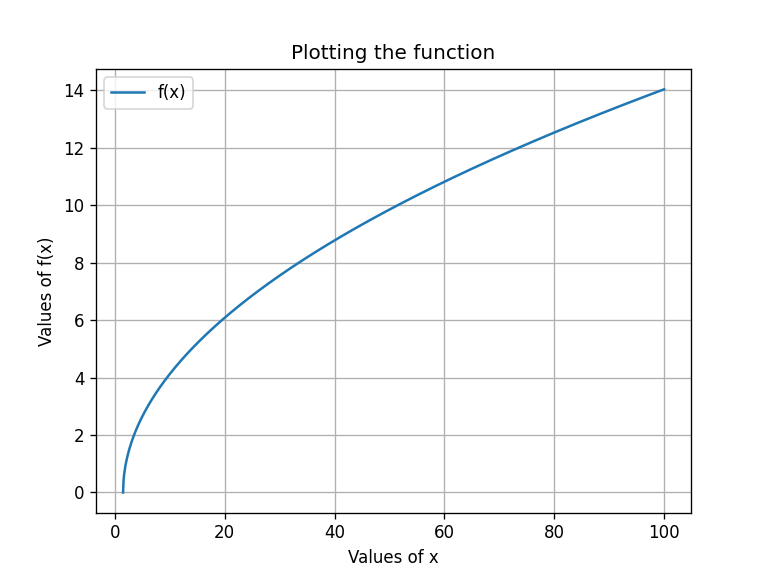
\includegraphics[width=\columnwidth]{Fig_1.png}
		\caption{Plotting the function, $f(x) = \sqrt{2x-3}$}
	\end{figure}\\
	We can clearly see, by drawing any horizontal straight line, we can't make the line touch the graph twice.\\
	$\therefore f(x)$ is an one to one, i.e., an injective function.
	\item
	\textbf{Verification for subjective function:}\\
	We can verify, if the function is strictly increasing or decreasing by taking its \underline{"Derivative test"} with respect to 'x'.\\
	Given,
	\begin{align}
		 f(x) = \sqrt{2x-3}
\end{align}
Differentiating on both sides with respect to $'x'$,
\begin{align}
\frac{df(x)}{dx} = \frac{d}{dx}\sqrt{2x-3}
\end{align}
\begin{align}
\frac{df(x)}{dx} = \frac{1}{2\sqrt{2x-3}}(2)
\end{align}
\begin{align}
\therefore\frac{df(x)}{dx} = \frac{1}{\sqrt{2x-3}}
\end{align}
Since, we know that $\sqrt{2x-3}$ is always positive. Therefore, this implies that $\frac{df(x)}{dx}$ is always positive.\\
\begin{align}
\frac{1}{\sqrt{2x-3}} > 0
\end{align}
\begin{align}
\therefore\frac{df(x)}{dx} > 0
\end{align}
Hence, we can say that the function, f(x) is always increasing. Therefore, f(x) covers all the values of its co-domain.\\
$\therefore f(x)$ is an onto, i.e., a subjective function.
	\end{itemize}
	\item
	\textbf{\underline{Finding the inverse of the function:}}\\
	Since, we found out that the function, f(x) is a bijective function (both injective and subjective). Therefore, its inverse exists.\\
	We can find the inverse of the function, by swapping $x$ with $f^{-1}(x)$ and $f(x)$ with $x$. Hence we get,
	\begin{align}
	x = \sqrt{2(f^{-1}(x)) - 3}
	\end{align}
	\begin{align}
	x^{2} = 2(f^{-1}(x)) - 3
	\end{align}
	\begin{align}
	\therefore f^{-1}(x) = \frac{x^{2} + 3}{2}
	\end{align}
	We can even verify, the above obtained inverse function by plotting and checking an inverse function property.\\
	\textbf{Inverse function property:} It states that, the original function$(f(x))$ and its inverse$(f^{-1}(x))$ are always mirror images in the line, y = x.
	\end{itemize}
\end{document}